\documentclass[10pt]{book}

%These tell TeX which packages to use.
\usepackage{array,epsfig}
\usepackage{amsmath}
\usepackage{amsfonts}
\usepackage{amssymb}
\usepackage{amsxtra}
\usepackage{amsthm}
\usepackage{mathrsfs}
\usepackage{color}
\usepackage{enumitem}
%\usepackage{mdframed}
\usepackage[most]{tcolorbox}
\usepackage{pgfplots}
\usetikzlibrary{arrows}
\pgfplotsset{compat=1.6}

\pgfplotsset{soldot/.style={color=black,only marks,mark=*}} \pgfplotsset{holdot/.style={color=black,fill=white,only marks,mark=*}}

%Here I define some theorem styles and shortcut commands for symbols I use often
\theoremstyle{definition}
\newtheorem{defn}{Definition}
\newtheorem{thm}{Theorem}
\newtheorem{cor}{Corollary}
\newtheorem*{rmk}{Remark}
\newtheorem{lem}{Lemma}
\newtheorem*{joke}{Joke}
\newtheorem{ex}{Example}
\newtheorem*{soln}{Solution}
\newtheorem{prop}{Proposition}

\newcommand{\lra}{\longrightarrow}
\newcommand{\ra}{\rightarrow}
\newcommand{\surj}{\twoheadrightarrow}
\newcommand{\graph}{\mathrm{graph}}
\newcommand{\bb}[1]{\mathbb{#1}}
\newcommand{\Z}{\bb{Z}}
\newcommand{\Q}{\bb{Q}}
\newcommand{\R}{\bb{R}}
\newcommand{\C}{\bb{C}}
\newcommand{\N}{\bb{N}}
\newcommand{\M}{\mathbf{M}}
\newcommand{\m}{\mathbf{m}}
\newcommand{\MM}{\mathscr{M}}
\newcommand{\HH}{\mathscr{H}}
\newcommand{\Om}{\Omega}
\newcommand{\Ho}{\in\HH(\Om)}
\newcommand{\bd}{\partial}
\newcommand{\del}{\partial}
\newcommand{\bardel}{\overline\partial}
\newcommand{\textdf}[1]{\textbf{\textsf{#1}}\index{#1}}
\newcommand{\img}{\mathrm{img}}
\newcommand{\ip}[2]{\left\langle{#1},{#2}\right\rangle}
\newcommand{\inter}[1]{\mathrm{int}{#1}}
\newcommand{\exter}[1]{\mathrm{ext}{#1}}
\newcommand{\cl}[1]{\mathrm{cl}{#1}}
\newcommand{\ds}{\displaystyle}
\newcommand{\vol}{\mathrm{vol}}
\newcommand{\cnt}{\mathrm{ct}}
\newcommand{\osc}{\mathrm{osc}}
\newcommand{\LL}{\mathbf{L}}
\newcommand{\UU}{\mathbf{U}}
\newcommand{\support}{\mathrm{support}}
\newcommand{\AND}{\;\wedge\;}
\newcommand{\OR}{\;\vee\;}
\newcommand{\Oset}{\varnothing}
\newcommand{\st}{\ni}
\newcommand{\wh}{\widehat}
%Pagination stuff.
\setlength{\topmargin}{-0.75in}
\setlength{\oddsidemargin}{0in}
\setlength{\evensidemargin}{0in}
\setlength{\textheight}{9.in}
\setlength{\textwidth}{6.5in}
\pagestyle{empty}
\begin{document}
\begin{flushleft}
Name:\underline{\hspace{13cm}}Date:\underline{\hspace{2cm}}
\end{flushleft}
\begin{center}
{\Large Math 1041-012 \hspace{0.5cm} Section 4.7}
\end{center}
%\vspace{0.2 cm}

\begin{tcolorbox}
\subsection*{Steps In Solving Optimization Problems}
\begin{enumerate}
    \item Identify quantities that are fixed and quantities that are variable. Is it a maximizing problem or a minimizing problem?
    \item Draw and label a diagram if possible. Assign symbols to variables.
    \item Relate the variables, there is a formula (or two formulas) that go with the diagram you drew. There maybe too many variables, some how you need to relate them together to reduce the number of variables. If possible find the domain. 
    \item Use calculus to find the absolute Max or Min: Closed Interval Method, First Derivative Test or Second Derivative Test.
\end{enumerate}
\end{tcolorbox}
\subsection*{Example 1: Mathy Example}
Find two positive numbers whose sum is 20 and whose product is as large as possible?
\begin{enumerate}[label=(\alph*)]
    \item Do we want to maximize or minimize a quantity? How do you know?
    \item Write down two formulas that are implied by the problem.\vspace{2cm}
    \item Reduce the number of variables by solving for one variable in terms of the other to get a new formula.\vspace{3cm}
    \item What is the \textit{domain} of the formula from above?\vspace{1cm}
    \item Take the derivative and find the maximum/minimum.
\end{enumerate}
\clearpage
\subsection*{Example 2: Fence Problem}
A farmer has 2400 feet of fencing and wants to fence off a rectangular field that borders a straight river. He wants no fence along the river. What are the dimensions of the field that has the largest area?
\begin{enumerate}[label=(\alph*)]
    \item Do we want to maximize or minimize a quantity? How do you know?
    \item Make a rough sketch of the problem.\vspace{4cm}
    \item Write down two formulas that are implied by the problem.\vspace{2cm}
    \item Reduce the number of variables by solving for one variable in terms of the other to get a new formula.\vspace{3cm}
    \item What is the \textit{domain} of the formula from above?\vspace{1cm}
    \item Take the derivative and find the maximum/minimum.
\end{enumerate}
\clearpage
\subsection*{Example 3: You Try} You purchased 1200 feet of steel fencing to close off a rectangular section of land on all four sides. What is the largest area you can enclose? And what are the dimensions to this largest rectangular area?
\clearpage
\subsection*{Example 4: Cylindrical Can}
A cylindrical can is to be made to hold 1 liter of oil. Find the dimensions of the can that will minimize the cost of the metal manufacture the can.
\clearpage
\subsection*{Example 5: Using Distance}
Find the point on the parabola $y^2=2x$ that is closest to the point $(1,4)$.
\begin{figure}[h!]
    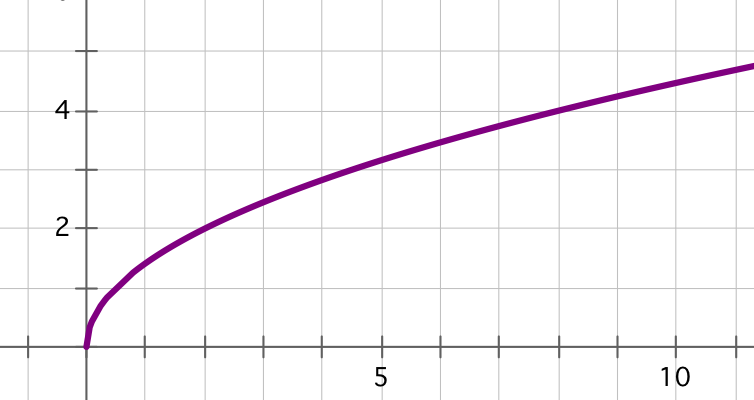
\includegraphics[width=7cm]{distprob.png}
\end{figure}
\end{document}